\documentclass[border=12pt]{standalone}
\usepackage{tikz}
\usetikzlibrary{shapes.geometric, arrows.meta, positioning, calc, fit, backgrounds}
\usepackage{fontspec}
\usepackage{amsmath}
\setmainfont{DejaVu Sans}

\begin{document}
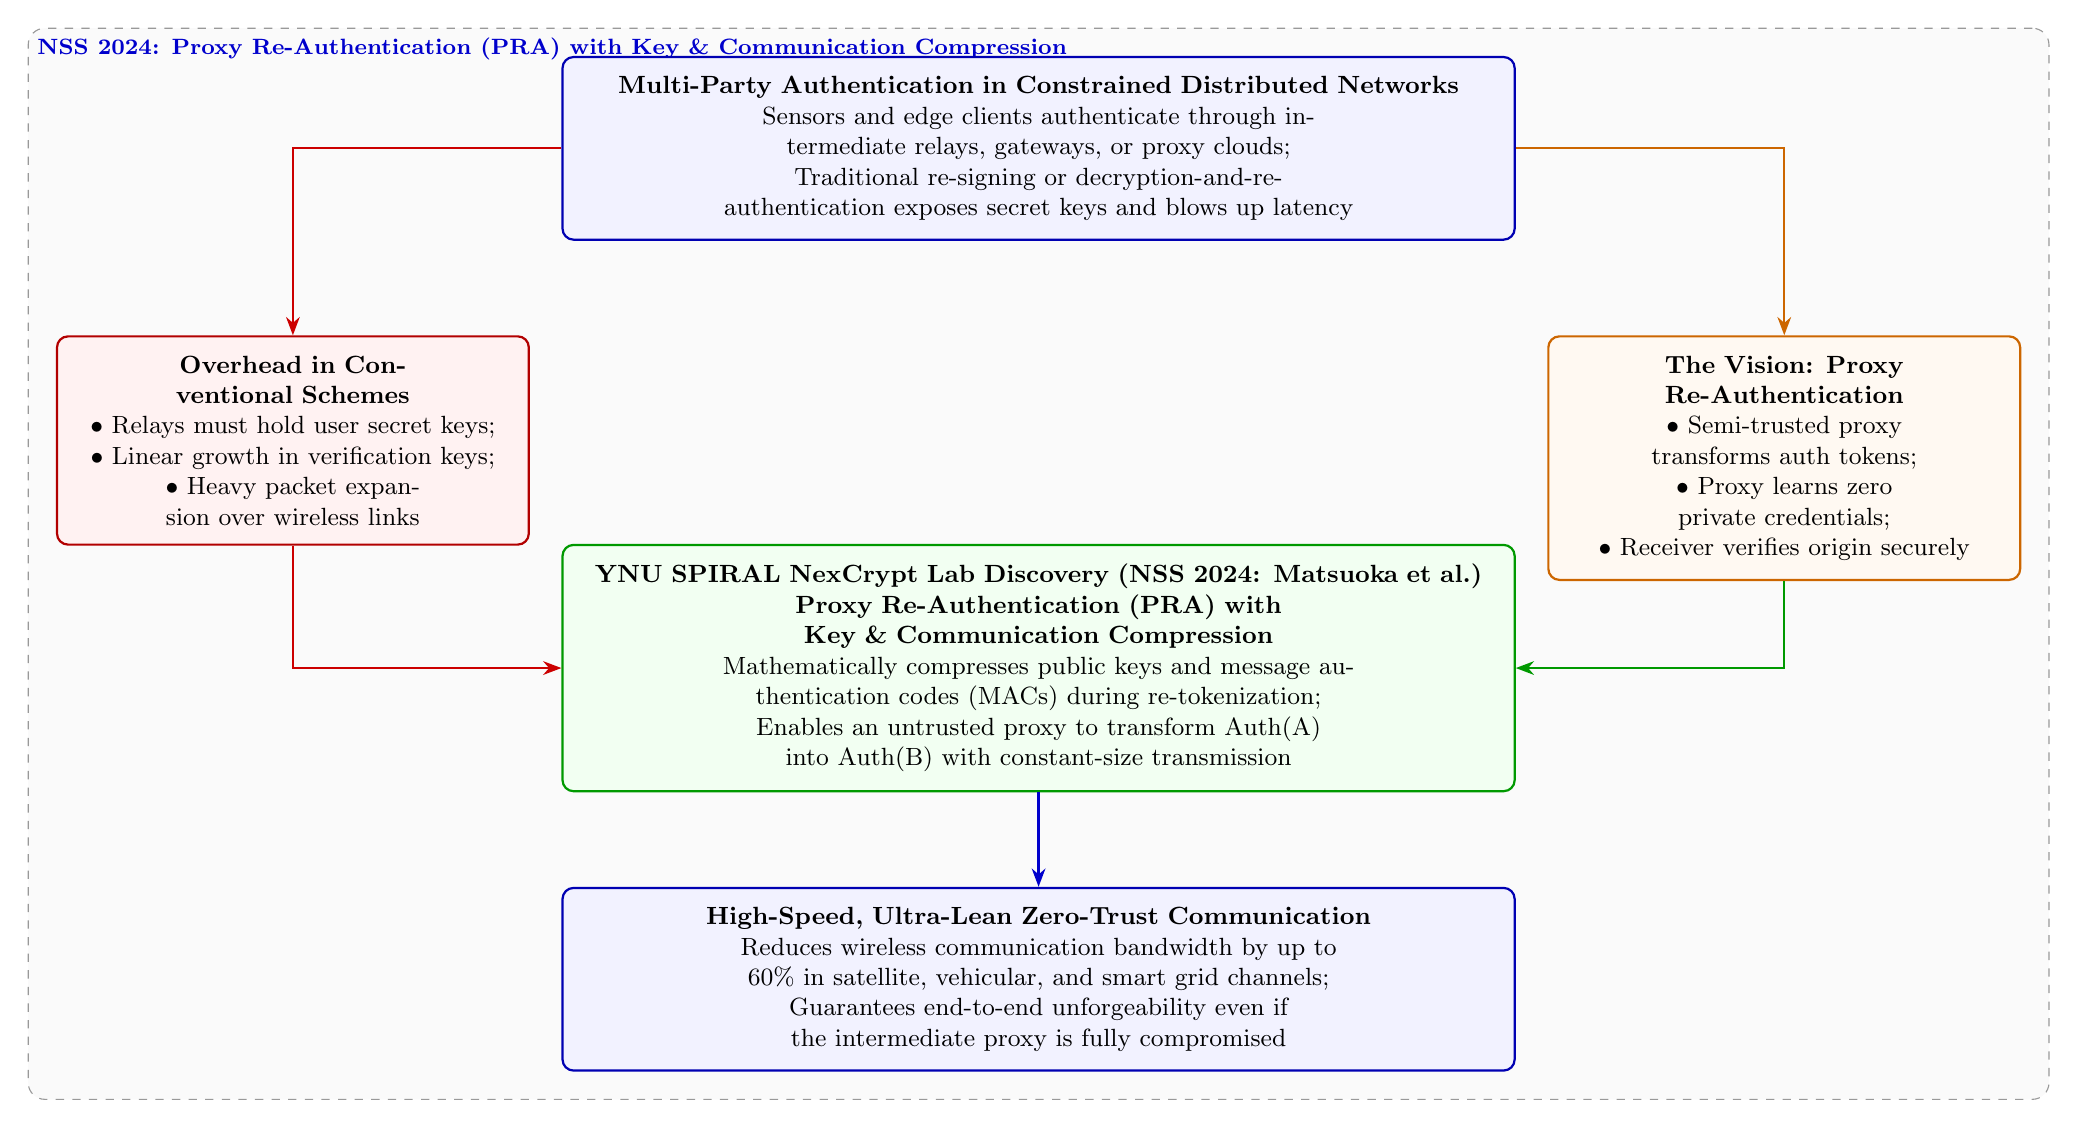
\begin{tikzpicture}[
    font=\small,
    >=Stealth,
    node distance=1.2cm,
    block/.style={rectangle, draw=blue!70!black, fill=blue!5, rounded corners=4pt, thick, align=center, inner sep=7pt},
    alertblock/.style={rectangle, draw=red!70!black, fill=red!5, rounded corners=4pt, thick, align=center, inner sep=7pt},
    greenblock/.style={rectangle, draw=green!60!black, fill=green!5, rounded corners=4pt, thick, align=center, inner sep=7pt},
    amberblock/.style={rectangle, draw=orange!80!black, fill=orange!5, rounded corners=4pt, thick, align=center, inner sep=7pt},
    groupbox/.style={draw=black!40, dashed, rounded corners=6pt, fill=black!2, inner sep=10pt}
]

    % Top: The Multi-Hop Authentication Bottleneck
    \node[block, text width=11.6cm] (problem) {\textbf{Multi-Party Authentication in Constrained Distributed Networks}\\Sensors and edge clients authenticate through intermediate relays, gateways, or proxy clouds;\\Traditional re-signing or decryption-and-re-authentication exposes secret keys and blows up latency};

    % Left: Key & Bandwidth Bloat
    \node[alertblock, below left=1.2cm and 0.4cm of problem, text width=5.5cm] (overhead) {\textbf{Overhead in Conventional Schemes}\\$\bullet$ Relays must hold user secret keys;\\$\bullet$ Linear growth in verification keys;\\$\bullet$ Heavy packet expansion over wireless links};

    % Right: Proxy Re-Encryption Concept
    \node[amberblock, below right=1.2cm and 0.4cm of problem, text width=5.5cm] (concept) {\textbf{The Vision: Proxy Re-Authentication}\\$\bullet$ Semi-trusted proxy transforms auth tokens;\\$\bullet$ Proxy learns zero private credentials;\\$\bullet$ Receiver verifies origin securely};

    \draw[->, thick, red!80!black] (problem) -| (overhead);
    \draw[->, thick, orange!80!black] (problem) -| (concept);

    % Middle: YNU Discovery (NSS 2024: Matsuoka, Chiku, Hara, Shikata)
    \node[greenblock, below=1.2cm of $(overhead)!0.5!(concept)$, text width=11.6cm] (breakthrough) {\textbf{YNU SPIRAL NexCrypt Lab Discovery (NSS 2024: Matsuoka et al.)}\\\textbf{Proxy Re-Authentication (PRA) with Key \& Communication Compression}\\Mathematically compresses public keys and message authentication codes (MACs) during re-tokenization;\\Enables an untrusted proxy to transform Auth(A) into Auth(B) with constant-size transmission};

    \draw[->, thick, red!80!black] (overhead) |- (breakthrough);
    \draw[->, thick, green!60!black] (concept) |- (breakthrough);

    % Bottom: Impact
    \node[block, below=1.2cm of breakthrough, text width=11.6cm] (impact) {\textbf{High-Speed, Ultra-Lean Zero-Trust Communication}\\Reduces wireless communication bandwidth by up to 60\% in satellite, vehicular, and smart grid channels;\\Guarantees end-to-end unforgeability even if the intermediate proxy is fully compromised};

    \draw[->, thick, blue!80!black] (breakthrough) -- (impact);

    \begin{scope}[on background layer]
        \node[groupbox, fit=(problem) (overhead) (concept) (breakthrough) (impact), label={[anchor=north west, font=\footnotesize\bfseries, blue!80!black]north west:NSS 2024: Proxy Re-Authentication (PRA) with Key \& Communication Compression}] {};
    \end{scope}

\end{tikzpicture}
\end{document}
